\thispagestyle{empty}

\begin{center}
\begin{spacing}{1}

\begin{figure}[H]
    \centering
    
\includegraphics{images/titul/1.png} %[width=0.15\linewidth]
\end{figure}


        \small МИНОБРНАУКИ РОССИИ\\
        \small Федеральное государственное бюджетное образовательное учреждени\\
        \small высшего образования\\
        \small \textbf{«МИРЭА – Российский технологический университет}»\\
        \Large\textbf{РТУ МИРЭА}
        \vspace{0cm}
        
    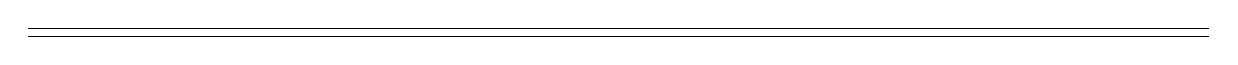
\begin{tikzpicture}
    \draw(0,0) -- (15,0);
    \draw(0,0.1) -- (15,0.1);
    \end{tikzpicture}



        \normalsize  Филиал РТУ МИРЭА в г. Фрязино\\
        \normalsize Базовая кафедра №143 – конструирования СВЧ и цифровых радиоэлектронных средств\\
        
        \vspace{0.5cm} 
        
        \Large\textbf{КУРСОВАЯ РАБОТА}\\
        \normalsize по дисциплине\\
        \normalsize <<Основы теории радиоэлектронных устройств>>\\
        \textbf{Тема курсовой работы: «ППМ для АФАР Х-диапазона с предельно низким уровнем боковых лепестков: -50 dB»}

        \vspace{2cm}


    \begin{flushleft} Студент группы: \hspace{0.5cm} \underline{ФКМО-01-22} \hspace{2cm} Бадулин Д.Р. \end{flushleft}
    \vspace{0.3cm}
    \begin{flushleft} Руководитель курсового проекта \hspace{2cm} Куприянов П.В. \end{flushleft}
    \begin{flushleft} Профессор, д.т.н.	 \end{flushleft}
    \vspace{0.3cm}
    \begin{flushleft} Рецензент \end{flushleft}
    \vspace{0.5cm}
    \begin{flushleft} Работа представлена к защите \hspace{0.3cm}  \data \end{flushleft}
    \vspace{0.5cm}
    \begin{flushleft} Допущен к защит \hspace{0.3cm}   \data \end{flushleft}
    \vspace{2cm}


\normalsize Фрязино \the\year{}
\end{spacing}
\end{center}


\newpage
\thispagestyle{empty} 

\begin{center}
\begin{spacing}{1}
    \begin{figure}[H]
        \centering
        
\includegraphics{images/titul/1.png} %[width=0.15\linewidth]
    \end{figure}


    \small МИНОБРНАУКИ РОССИИ\\
    \normalsize Федеральное государственное бюджетноеобразовательное учреждени\\
    \normalsize высшего образования\\
    \normalsize \textbf{«МИРЭА – Российский технологический университет}»\\
    \Large\textbf{РТУ МИРЭА}\\
        
    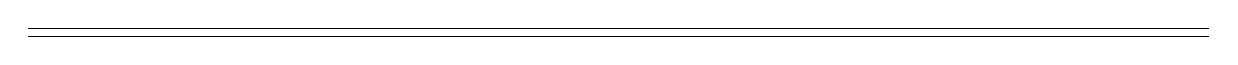
\begin{tikzpicture}
    \draw(0,0) -- (15,0);
    \draw(0,0.1) -- (15,0.1);
    \end{tikzpicture}




    \normalsize  Филиал РТУ МИРЭА в г. Фрязино\\
    \normalsize Базовая кафедра №143 – конструирования СВЧ и цифровых радиоэлектронных средств\\
    
    

    \begin{flushright}
        \small    \textbf{Утверждаю}\\
        \footnotesize    Заведующий кафедрой\\
        \footnotesize    Щербаков С.В.\\
        \footnotesize    \data
    \end{flushright}

    
    
    \large \textbf{ЗАДАНИЕ}\\
    \normalsize \textbf{на выполнение курсовой работы}\\
    \normalsize \textbf{по дисциплине «Основы теории радиоэлектронных устройств»}
    
    
    
    \end{spacing}
\end{center}

\begin{spacing}{1}
    \begin{enumerate}
        %\normalsize
        \footnotesize \item \textbf{Тема «ППМ для АФАР Х-диапазона с предельно низким уровнем боковых лепестков: -50 dB»}
        
        \item \textbf{Исходные данные:}\\
        Уровень боковых лепестков: -50 дБ.
        
        \item  \textbf{Перечень вопросов, подлежащих разработке, и обязательного графического материала:}
         %\footnotesize
        Техническое задание на научно-исследовательскую работу, ТЗ должно включать в себя: 
        
требования назначения, требования живучести, требования надежности и стойкости к внешним воздействиям, требования гамма-процентной наработки до отказа, требования наработки до отказа всей системы 1000 часов (2000 модулей в системе), требования технологичности: применяемые технологии, описание как подается питание физически, протокол управления; требования к документации.
        
        \item \textbf{Срок представления к защите курсового проекта:\\ до}  \data
    \end{enumerate}
    

    \begin{table}[H]
        \flushleft
        \begin{tabular}{ll}
            \begin{tabular}{l}
            \footnotesize    Задание на курсовую\\ \footnotesize работу выдал
            \end{tabular} & \footnotesize \data\\
            
            \begin{tabular}{l}
            \footnotesize    Задание на курсовую\\ \footnotesize работу получил
            \end{tabular} & \footnotesize \data\\
        
        \end{tabular}
    \end{table}
  
  
  
  \begin{center}
    \normalsize   Фрязино \the\year{}
  \end{center}
  
\end{spacing}
\newpage